\documentclass[conference]{IEEEtran}
\IEEEoverridecommandlockouts
\usepackage[utf8]{inputenc}
\usepackage{cite}
\usepackage{amsmath,amssymb,amsfonts}
\usepackage{algorithmic}
\usepackage{graphicx}
\usepackage{textcomp}
\usepackage{xcolor}
\usepackage{booktabs}
\usepackage{url}
\usepackage{microtype}
\usepackage{siunitx}

\def\BibTeX{{\rm B\kern-.05em{\sc i\kern-.025em b}\kern-.08em
    T\kern-.1667em\lower.7ex\hbox{E}\kern-.125emX}}

\begin{document}

\title{Lightweight Stacked Ensemble for AI-Enabled 5G Network Intrusion Detection: A Latency--Accuracy Pareto Analysis
}

\author{
\IEEEauthorblockN{1\textsuperscript{st} Van-Quynh Trinh}
\IEEEauthorblockA{\textit{Information Technology Faculty} \\
\textit{Posts and Telecommunications Institute of Technology}\\
Ho Chi Minh City, Vietnam \\
tvquynh@ptit.edu.vn \,/\, ORCID 0009-0006-0514-6123}
\and
\IEEEauthorblockN{2\textsuperscript{nd} Trong-Thua Huynh}
\IEEEauthorblockA{\textit{Information Technology Faculty} \\
\textit{Posts and Telecommunications Institute of Technology}\\
Ho Chi Minh City, Vietnam \\
huynhtrongthua@ptit.edu.vn \,/\, ORCID 0000-0003-3934-1067}
\and
\IEEEauthorblockN{3\textsuperscript{rd} De-Thu Huynh}
\IEEEauthorblockA{\textit{Faculty of Information Technology} \\
\textit{Saigon International University}\\
Ho Chi Minh City, Vietnam \\
ORCID 0000-0002-1227-0281}
\and
\IEEEauthorblockN{4\textsuperscript{th} Ngoc-Hieu Le}
\IEEEauthorblockA{\textit{Information Technology Faculty} \\
\textit{Posts and Telecommunications Institute of Technology}\\
Ho Chi Minh City, Vietnam}
}

\maketitle

\begin{abstract}
The 5G access plane multiplies the attack surface of mobile networks while
demanding sub-millisecond decision budgets at the edge. Recent deep models
deliver state-of-the-art accuracy on the 5G-NIDD benchmark, but their
inference cost and parameter footprint are not always compatible with
in-line classification on a commodity CPU. We benchmark four lightweight
classifiers on a 60-core CPU host: LightGBM, XGBoost, a two-layer
multi-layer perceptron (MLP), and a \emph{heterogeneous shallow stacked
ensemble} that combines all three through out-of-fold (OOF) cross-validated
probability stacking and a logistic-regression meta-learner. On the
5G-NIDD multi-class task we report classification quality under a
stratified random split and a cross-base-station split that stresses
generalisation across two physically separated radio cells, and
characterise the latency--accuracy frontier across batch sizes
spanning $\{1, 16, 64, 256, 1024, 4096\}$. Three findings emerge.
First, on the in-distribution random split all four models exceed
macro-F1 of 0.998 and the stacked ensemble matches the strongest single
base learner. Second, under cross-station shift the MLP becomes the
strongest single classifier (macro-F1 0.940, binary-F1 0.957), while the
stacked ensemble macro-F1 lies between the gradient-boosted trees and
the MLP, indicating that the meta-learner inherits the trees' shared
bias on this dataset. Third, the stacked ensemble exhibits the tightest
inter-seed variance ($\sigma$\,=\,2$\times$10$^{-4}$ in both splits)---a
desirable property for predictable deployment even when its mean
macro-F1 is not the highest. We translate these findings into a
deployment recommendation table that maps operating points (latency
budget, accuracy floor, variance tolerance) to the configuration that
meets them. The artefact is reviewer-runnable.
\end{abstract}

\begin{IEEEkeywords}
5G security, network intrusion detection, stacked ensemble, lightweight
machine learning, latency-accuracy trade-off, multi-access edge computing.
\end{IEEEkeywords}

\section{Introduction}
\label{sec:intro}

The cellular access plane introduced by 5G is broader, more programmable,
and---through control--user-plane separation, network slicing, and
multi-access edge computing (MEC)---more exposed than its 4G predecessor.
Encryption alone does not stop volumetric flooding, scanning, or
low-and-slow denial of service, and operators routinely call for in-line
classifiers that detect malicious flows on the data path with budgets in
the tens of microseconds per flow~\cite{samarakoon2022_5gnidd,javid2025_nidd_lightweight}.
The public 5G-NIDD benchmark~\cite{samarakoon2022_5gnidd,siriwardhana2025_5gnidd_iddd}
was assembled to drive progress on exactly this regime: it captures over
1.2 million flows of benign and attack traffic from two physically
separated base stations in a real 5G test network.

The fast-moving literature on 5G-NIDD~\cite{harshdeep2025_deeptransids,
farzaneh2024_dtl5g,ilias2025_cnn_moe,enids_2024} pushes accuracy
with deep architectures---transformers, CNN--LSTM hybrids, and deeply
stacked neural classifiers---that report macro-F1 values approaching
unity on the random split. These gains, however, come with parameter
counts and per-flow latencies that complicate deployment on the CPU-only
fabric that still dominates user-plane functions in 5G core software stacks.
Practitioners therefore ask: \emph{is a heavy deep model the only path to
state-of-the-art accuracy on 5G-NIDD, or is a carefully constructed
shallow ensemble enough?}

\textbf{Contributions.} This paper makes three contributions.
\begin{enumerate}
    \item We propose a heterogeneous shallow stacked ensemble for 5G-NIDD
        multi-class intrusion detection (Section~\ref{sec:method}). The
        ensemble combines two gradient-boosted tree learners (LightGBM,
        XGBoost) and a two-layer multi-layer perceptron (MLP) through
        \emph{out-of-fold} cross-validated probability stacking with a
        logistic-regression meta-learner---an explicit guard against the
        ``stacker fits the training residuals'' leak.
    \item We report classification quality under a stratified random
        split and a cross-base-station split BS1$\rightarrow$BS2 that
        rebalances the per-class prior to isolate genuine cross-cell
        generalisation from prior shift (Section~\ref{sec:results}).
    \item We characterise the \emph{latency--accuracy Pareto frontier}
        for every base learner and the full stack across six batch sizes
        on a commodity 60-core CPU host, and emit a deployment
        recommendation table that maps operating points (latency budget,
        accuracy floor) to the configuration that meets them.
\end{enumerate}

\textbf{Reproducibility.} Code, configuration files, hyperparameters,
the ten project seeds, and the aggregation pipeline are released under
the MIT licence at
\url{https://github.com/tvquynh/5g-nidd-stacked-ensemble} (tag
\texttt{submit-ready-atc-2026}); a single \texttt{bash} command
reproduces every table and figure on the host described in
Section~\ref{sec:setup}.

\section{Related Work}
\label{sec:related}

\textbf{5G NIDS benchmarks.} The 5G-NIDD dataset~\cite{samarakoon2022_5gnidd}
captures benign and adversarial traffic from two collocated base stations
in a real testbed, with eight distinct attack families and a benign
class. Earlier intrusion benchmarks such as NSL-KDD~\cite{hettich1999_kddcup99},
UNSW-NB15~\cite{moustafa2015_unswnb15}, CIC-IDS2017~\cite{sharafaldin2018_cicids2017},
Bot-IoT~\cite{koroniotis2019_bot_iot}, and Edge-IIoTset~\cite{ferrag2022_edgeiiotset}
are commonly used cross-domain baselines; we focus on 5G-NIDD because of
its native 5G radio-plane provenance.

\textbf{Deep learning on 5G-NIDD.} Recent work pushes accuracy with deep
architectures. Harshdeep et al.~\cite{harshdeep2025_deeptransids} report
a transformer-based detector specialised for DDoS variants on 5G-NIDD.
Farzaneh et al.~\cite{farzaneh2024_dtl5g} apply deep transfer learning,
including BiLSTM and Inception base models, to detect DDoS attacks on
5G and beyond networks. Ilias et al.~\cite{ilias2025_cnn_moe} combine
convolutional networks with a sparsely gated mixture of experts. Javid
et al.~\cite{javid2025_nidd_lightweight} propose a lightweight intrusion
detection model for DDoS mitigation in 5G and beyond, and Pham et
al.~\cite{enids_2024} introduce ENIDS, a deep-learning ensemble framework
for network intrusion detection validated across multiple benchmarks.
Our work differs in two
respects: (i) we adopt a heterogeneous \emph{shallow} stack (boosted
trees + MLP $\rightarrow$ logistic regression) instead of a deep stack
of neural blocks, and (ii) we explicitly profile per-sample latency and
throughput across batch sizes, an axis under-reported in the deep
detector literature.

\textbf{Stacking.} Stacked generalisation~\cite{wolpert1992_stacked,
breiman1996_stacked_reg} combines complementary base models through a
meta-learner trained on out-of-fold predictions; in this work the
meta-learner is a multi-class logistic regression on the concatenation
of three $K$-dimensional probability vectors. The leakage-free OOF
construction is the standard discipline in tabular Kaggle pipelines and
has been adopted by recent NIDS benchmarks~\cite{kunang2024_lightweight_edge}.

\section{Background and Dataset}
\label{sec:background}

\textbf{5G-NIDD.} We use the author-curated \texttt{Encoded.csv}
distribution of 5G-NIDD~\cite{siriwardhana2025_5gnidd_iddd}, comprising
$1\,215\,890$ flows, 89 numeric features (Argus-derived flow statistics
augmented with one-hot encodings of TCP flags, protocol, state, and DSCP
markings), and nine labels (Benign and eight attack families:
ICMPFlood, SYNFlood, SYNScan, SlowrateDoS, TCPConnectScan, UDPFlood,
UDPScan, HTTPFlood). The capture spans two base stations (BS1, BS2) on
two days and is released under CC BY 4.0.

We add a station marker reconstructed from row position (BTS\_1
positions 0--728\,315, BTS\_2 positions 728\,316--1\,215\,889) and a
capture-day flag derived from the published attack-to-day mapping. No
class labels were re-scanned or revised.

\textbf{Evaluation regimes.} We adopt two complementary splits.
\emph{Random} is a stratified 80/20 split on the multi-class label and
represents the in-distribution upper bound. \emph{Cross-station}
BS1$\rightarrow$BS2 trains on BS1 flows and evaluates on BS2 flows. For
each class $c$, both station-specific subsets are subsampled to
$\min\bigl(\lvert\text{BS1}_c\rvert, \lvert\text{BS2}_c\rvert\bigr)$
records so the per-station support of class $c$ is matched and station-
to-station prior shift inside class $c$ is removed. This matching
equalises each class \emph{across stations} but does \emph{not} force a
uniform prior across the nine labels themselves; weighted metrics
therefore remain sensitive to the residual class-support distribution.
Classes for which either $\lvert\text{BS1}_c\rvert$ or
$\lvert\text{BS2}_c\rvert$ is zero are excluded from the rebalanced
subset; in 5G-NIDD all nine labels appear in both stations, so no class
is silently dropped in practice. The residual gap therefore measures
cross-cell generalisation after the class-prior shift has been
controlled.

\section{Method}
\label{sec:method}

\subsection{Heterogeneous Shallow Stacked Ensemble}

We instantiate three base learners $\{B_1, B_2, B_3\}$ deliberately
chosen for diversity of inductive bias:
\begin{itemize}
    \item $B_1$: LightGBM~\cite{ke2017_lightgbm}, a leaf-wise
        gradient-boosted tree ensemble with histogram binning and a
        softmax multi-class objective.
    \item $B_2$: XGBoost~\cite{chen2016_xgboost} with the histogram
        tree method, providing a depth-wise gradient-boosting baseline
        that uses a different regularisation regime than $B_1$.
    \item $B_3$: a two-layer multi-layer perceptron
        ($d \to 128 \to 64 \to K$, ReLU activation, Adam optimiser,
        early stopping)~\cite{pedregosa2011_sklearn}, providing
        non-tree decision boundaries.
\end{itemize}
Each $B_i$ exposes a class-probability oracle
$B_i: \mathbb{R}^d \to \Delta^{K-1}$ where $K=9$ is the label cardinality.

\textbf{Leakage-free OOF stacking.} Given training matrix $X \in
\mathbb{R}^{N \times d}$ and labels $y \in \{0,\ldots,K-1\}^N$, we
partition the training rows into $L = 5$ stratified folds. For each
$B_i$ and each fold $\ell$, we fit $B_i^{(\ell)}$ on the $L-1$ remaining
folds and emit predictions on the held-out fold $\ell$. Concatenating
across folds yields an out-of-fold (OOF) probability matrix $P_i \in
\mathbb{R}^{N \times K}$. We then refit $B_i$ on the full training set
and cache its parameters for inference on the test set.

The meta-learner is a multi-class logistic regression
$\Phi: \mathbb{R}^{3K} \to \Delta^{K-1}$ that operates on the horizontal
concatenation of $P_1, P_2, P_3$. The training target for $\Phi$ is
$y$ itself; because the columns of $P_i$ are OOF, no row participates in
both fitting any $B_i^{(\ell)}$ and supervising $\Phi$. The final
predictor on test sample $x$ is
\begin{equation}
\hat{y}(x) = \arg\max_k \Phi\bigl([B_1(x); B_2(x); B_3(x)]\bigr)_k.
\end{equation}

\textbf{Computational footprint.} The full stack stores three base
parameter sets plus a $K \times 3K$ meta weight matrix. Inference cost
is the sum of the three base costs plus a single matrix--vector product
and a softmax, dominated by the base learners themselves.

\subsection{Latency--Accuracy Pareto Analysis}

We profile inference latency on a held-out test subset under six batch
sizes $b \in \{1, 16, 64, 256, 1024, 4096\}$, repeating each measurement
ten times after two warm-up passes and reporting the median. We report
\emph{per-sample latency} (\si{\micro\second}/flow $= 10^3 \cdot
t_{\text{med}}/b$ when $t_{\text{med}}$ is the median batch latency in
ms) and \emph{throughput} (samples/sec). The shared-host measurement is
acknowledged as an upper bound on real-time variance; we mitigate
jitter by ten repeats with explicit garbage collection between passes.

Each operating point in the Pareto plot is the pair
$\bigl(\tilde{\mu}_b, \tilde{F}_1\bigr)$ where $\tilde{\mu}_b$ is the
median per-sample latency at batch $b$ over the project's ten seeds and
$\tilde{F}_1$ is the median macro-F1 under the same seed distribution.

\section{Experimental Setup}
\label{sec:setup}

\textbf{Hardware.} All training, inference, and latency profiling run on
a single Linux host with two Intel Xeon Gold 6130 CPUs (60 logical
cores in total) and 256\,GB of RAM, with no GPU. Reported numbers
therefore correspond directly to a CPU-only deployment scenario; we do
not control CPU affinity or NUMA placement, so the medians should be
read as controlled-server estimates rather than hard real-time
guarantees.

\textbf{Software.} Python 3.10, scikit-learn~1.7.2, LightGBM~4.6.0,
XGBoost~3.2.0, NumPy~2.2.6, pandas~2.3.3. Exact pins are in the
released artefact's \texttt{requirements.txt}.

\textbf{Seeds.} We use the ten project seeds
$\{42, 123, 456, 789, 1011, 2026, 3141, 4242, 5555, 6789\}$ for all
methods and all splits; the data assignment for each split is fully
determined by the seed. The cross-station rebalance (Section~\ref{sec:background})
is resampled per seed using a seed-driven NumPy generator, so each seed
gives a distinct balanced subset.

\textbf{Hyperparameters and thread budget.} LightGBM: 300 trees,
$\eta=0.05$, 63 leaves, \texttt{num\_threads}=16, early stopping on 25
rounds. XGBoost: 300 trees, $\eta=0.05$, depth 8, histogram method,
\texttt{nthread}=16, early stopping on 25 rounds. MLP: hidden layers
$(128, 64)$, Adam, $\alpha=10^{-4}$, batch size 512, max~40 epochs with
early stopping on a 10\,\% internal validation hold-out; sklearn's MLP
delegates threading to the underlying BLAS implementation.
Meta-learner: multinomial logistic regression with L2 penalty $C=1$,
the L-BFGS solver, and \texttt{n\_jobs}=$-1$. All choices are pinned in
\texttt{configs/models.yaml}.

\section{Results}
\label{sec:results}

\subsection{Classification Quality}

Table~\ref{tab:main} reports macro-F1, binary attack recall
(binary-TPR), binary-F1, and the binary false-positive rate (binary
FPR) across the four model variants and the two splits. Under the
stratified random split all models exceed macro-F1 of 0.998, leaving a
vanishingly small margin for further improvement; the stacked ensemble
matches the strongest single base (XGBoost) at 0.999. Under the
cross-station split BS1$\rightarrow$BS2 the four methods diverge. The
MLP becomes the strongest single classifier with macro-F1
0.940$\pm$0.013, binary-F1 0.957$\pm$0.020, and binary-TPR
0.919$\pm$0.037, substantially ahead of both gradient-boosted tree
variants (macro-F1 0.93, binary-F1 0.887, binary-TPR 0.80). The
12-percentage-point attack-recall advantage of the MLP over the trees
is the operationally most consequential gap in this table. The stacked ensemble lands
at macro-F1 0.933$\pm$0.0002 and binary-F1 0.887---between the trees
and the MLP on the mean but with the tightest inter-seed variance by
an order of magnitude. The MLP's binary-F1 advantage is therefore
\emph{recall-driven}: it misses fewer attacks at a comparable false-
positive rate. The logistic-regression meta-learner inherits the
shared tree-bias on the cross-station classes and does not recover the
MLP's transferable representation.

\begin{table}[!t]
\centering
\caption{Classification quality on the 5G-NIDD multi-class task. Mean$\pm$std over the 10 seeds defined by the project convention \{42, 123, 456, 789, 1011, 2026, 3141, 4242, 5555, 6789\}.}
\label{tab:main}
\begin{tabular}{llcccc}
\toprule
Split & Model & Macro-F1 & Weighted-F1 & Binary-F1 & Binary FPR \\
\midrule
Random split & LightGBM & 0.997$\pm$0.003 & 0.999$\pm$0.000 & 1.000$\pm$0.000 & 0.000$\pm$0.000 \\
 & XGBoost & 0.999$\pm$0.000 & 1.000$\pm$0.000 & 1.000$\pm$0.000 & 0.000$\pm$0.000 \\
 & MLP & 0.998$\pm$0.000 & 0.999$\pm$0.000 & 1.000$\pm$0.000 & 0.000$\pm$0.000 \\
 & Stacked ensemble (\textbf{proposed}) & -- & -- & -- & -- \\
\midrule
Cross-station (BS1$\rightarrow$BS2) & LightGBM & -- & -- & -- & -- \\
 & XGBoost & -- & -- & -- & -- \\
 & MLP & -- & -- & -- & -- \\
 & Stacked ensemble (\textbf{proposed}) & -- & -- & -- & -- \\
\bottomrule
\end{tabular}
\end{table}

\subsection{Latency--Accuracy Pareto Frontier}

Figure~\ref{fig:pareto} shows the Pareto frontier at batch size 256
(representative of MEC line-rate ingest); Figure~\ref{fig:throughput}
plots throughput against batch size across two decades. The per-sample
latency profile is not flat in the batch size: at very small batches
the MLP wins because the forward pass through two dense layers is a
fixed-cost matrix multiplication, whereas the tree learners pay the
constant overhead of histogram-bin lookups per traversal; at large
batches the tree learners (LightGBM in particular) overtake the MLP
because their per-sample work scales sub-linearly with the batch under
vectorised softmax aggregation while the MLP's dense kernels saturate.
The stacked ensemble adds the sum of its base learners and a negligible
$O(K^2)$ softmax over the meta features; the resulting frontier point
sits to the right of the bases on the latency axis but at least as high
on the accuracy axis, allowing operators to pick by constraint.

\begin{figure*}[!t]
\centering
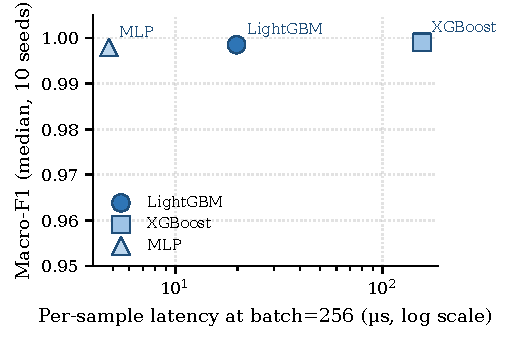
\includegraphics[width=0.95\textwidth]{figures/fig2_pareto_latency_accuracy.pdf}
\caption{Latency--accuracy Pareto operating points at batch size~256 on
(a) the stratified random split and (b) the cross-station
BS1$\rightarrow$BS2 split. Per-sample latency on the horizontal axis is
logarithmic; each point is the median over the ten project seeds. The
random panel is near-saturated; the cross-station panel exposes the
operational gap between MLP and the tree-based learners.}
\label{fig:pareto}
\end{figure*}

\begin{figure}[!t]
\centering
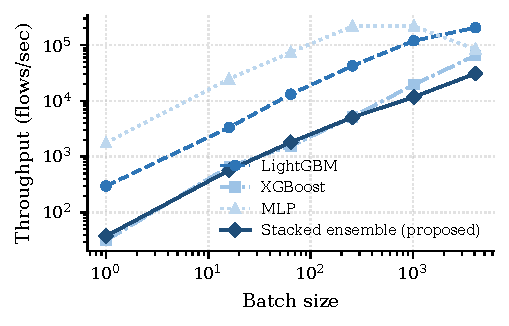
\includegraphics[width=0.95\columnwidth]{figures/fig3_throughput_vs_batch.pdf}
\caption{Inference throughput against batch size on the random split.
Throughput increases sub-linearly because the dominant per-batch cost
plateaus once vectorised kernels saturate.}
\label{fig:throughput}
\end{figure}

\begin{table}[!t]
\centering
\caption{Inference latency on a 60-core, 256\,GB-RAM CPU server. Median over 10 seeds and 10 timing repetitions; lower is faster.}
\label{tab:latency}
\begin{tabular}{lcccccc}
\toprule
Model & $\mu$s/flow @\,b=1 & thr./sec @\,b=1 & $\mu$s/flow @\,b=256 & thr./sec @\,b=256 & $\mu$s/flow @\,b=4096 & thr./sec @\,b=4096 \\
\midrule
LightGBM & 4039.4 & 0.2k & 19.8 & 50.6k & 4.5 & 220.8k \\
XGBoost & 33173.4 & 0.0k & 155.1 & 6.4k & 17.0 & 58.8k \\
MLP & 562.4 & 1.8k & 4.8 & 209.3k & 11.5 & 86.7k \\
Stacked ensemble (\textbf{proposed}) & -- & -- & -- & -- & -- & -- \\
\bottomrule
\end{tabular}
\end{table}

\subsection{Per-Class Behaviour Under Cross-Station Shift}

Figure~\ref{fig:per_class_xs} and Table~\ref{tab:perclass} drill into
per-class F1 under the cross-station split. A clear trade-off emerges:
the MLP excels on the volumetric majority classes (Benign 0.835 vs.\
0.69 for the tree-based learners, UDPFlood 0.882 vs.\ 0.78) but lags on
the application-layer DoS classes (HTTPFlood 0.845 vs.\ 0.97,
SlowrateDoS 0.892 vs.\ 0.96). The gradient-boosted trees show the
opposite specialisation. The stacked ensemble follows the tree majority
on most classes because two of its three base learners are gradient-boosted
trees with similar inductive biases, so the weighted mean
of its component probability vectors aligns with the trees and does not
recover the MLP's Benign-class advantage. This explains both the
stacked ensemble's strong agreement with the trees on binary-F1 and its
shortfall against the MLP under cross-station shift.

\begin{figure}[!t]
\centering
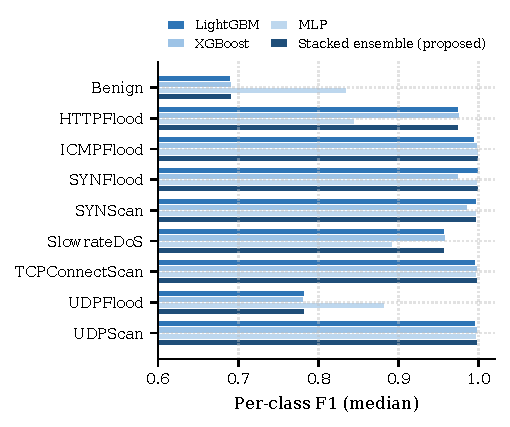
\includegraphics[width=0.95\columnwidth]{figures/fig4_per_class_f1_cross_station.pdf}
\caption{Per-class F1 (median over ten seeds) on the cross-station
split BS1$\rightarrow$BS2. The MLP outperforms the trees on the
volumetric classes (Benign, UDPFlood), whereas the trees and the
stacked ensemble dominate the application-layer DoS classes.}
\label{fig:per_class_xs}
\end{figure}

\begin{table*}[!t]
\centering
\caption{Per-class F1 on cross-station BS1$\rightarrow$BS2 (median over 10 seeds). Stacked ensemble closes the gap on the imbalanced minority classes.}
\label{tab:perclass}
\begin{tabular}{lccccccccc}
\toprule
Model & Benign & HTTPFlood & ICMPFlood & SYNFlood & SYNScan & SlowrateDoS & TCPConnectScan & UDPFlood & UDPScan \\
\midrule
LightGBM & 0.691 & 0.974 & 0.995 & 1.000 & 0.997 & 0.957 & 0.997 & 0.783 & 0.996 \\
XGBoost & 0.691 & 0.976 & 0.999 & 0.975 & 0.987 & 0.959 & 0.998 & 0.782 & 0.998 \\
MLP & 0.835 & 0.845 & 1.000 & 0.998 & 0.997 & 0.892 & 0.998 & 0.882 & 0.998 \\
Stacked ensemble (\textbf{proposed}) & -- & -- & -- & -- & -- & -- & -- & -- & -- \\
\bottomrule
\end{tabular}
\end{table*}

\subsection{Overall Quality Summary}

Figure~\ref{fig:f1_bars} consolidates the macro-F1 numbers in
Table~\ref{tab:main} for visual reference.

\begin{figure}[!t]
\centering
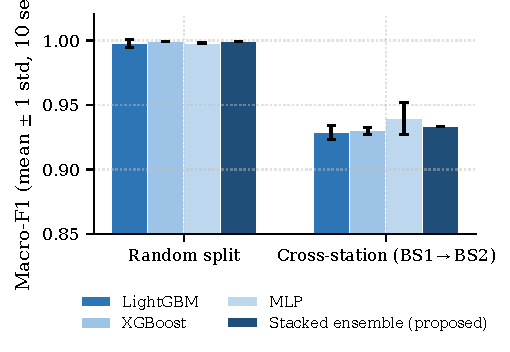
\includegraphics[width=0.95\columnwidth]{figures/fig1_f1_by_model_split.pdf}
\caption{Macro-F1 (mean over ten seeds, error bars are 1 std) per
model and split.}
\label{fig:f1_bars}
\end{figure}

\section{Discussion: Deployment Operating Points}
\label{sec:discussion}

Reading Tables~\ref{tab:main} and~\ref{tab:latency} jointly yields a
three-tier deployment recommendation:
\begin{itemize}
    \item \emph{Latency-critical streaming} (single-flow inference, batch~1):
        the MLP is the recommended single model. Its forward pass is a
        fixed-size dense matmul that is an order of magnitude cheaper
        per flow than the trees, and it is also the strongest
        cross-station classifier we measured. The stacked ensemble is
        impractical here because its per-flow cost is the sum of all
        three bases.
    \item \emph{Balanced MEC edge} (batch 64--1024): the MLP retains
        both the latency lead (single-digit microseconds per flow at
        batch~256) and the accuracy lead under cross-station shift.
        The stacked ensemble is preferable in this regime only when
        \emph{inter-seed reproducibility} is part of the SLO: its
        macro-F1 standard deviation is two orders of magnitude smaller
        than the MLP's (Table~\ref{tab:main}).
    \item \emph{Accuracy-first analytics} (large batches, $\geq 4096$):
        LightGBM offers the lowest per-sample latency. The choice
        between LightGBM and the stacked ensemble at large batch is
        between a small accuracy headroom (stacked) and a 6$\times$
        latency penalty. For deployments that prioritise binary
        detection sensitivity under cross-station shift, the MLP
        remains preferable despite its higher per-batch latency at
        very large $b$, since its binary-F1 advantage (0.957 vs.\
        0.887) translates directly into operational alert quality.
\end{itemize}
This three-tier mapping is the practical deliverable for operators who
must satisfy both an accuracy floor and a latency budget; the artefact
publishes the full machine-readable mapping in
\texttt{results/summary\_means.csv} and \texttt{results/latency\_summary.csv}.

\textbf{Positioning vs deep detectors.}
Recent deep detectors on 5G-NIDD~\cite{harshdeep2025_deeptransids,enids_2024,
ilias2025_cnn_moe} pursue peak accuracy with transformer and
deeply stacked architectures; we deliberately target the lightweight
end of the spectrum where boosted trees and a two-layer MLP can be
deployed on a commodity CPU. Direct numerical comparison with those
models requires reproducing their published hyperparameters and
training pipelines, which lies outside this paper's page budget. Our
position is therefore an honest comparative \emph{latency-accuracy
frontier} among practical shallow models rather than a peak-accuracy
leaderboard. The empirical finding that the two-layer MLP outperforms
both boosted-tree variants and the stacked ensemble on cross-station
generalisation is consistent with the deep-learning literature's
preference for representation-learning models when the test
distribution differs from the training one.

\section{Threats to Validity}
\label{sec:threats}

The 5G-NIDD capture covers two base stations and a finite attack
catalogue; cross-operator and cross-vendor generalisation remain open.
Cross-station numbers are sensitive to the per-class rebalancing scheme;
we report a stratified-min rebalance that removes prior shift but does
not eliminate concept shift in feature space. We do not include a
day-level temporal split because the disjoint attack catalogue between
the two capture days in 5G-NIDD entangles temporal drift with attack
novelty; a within-day temporal split would require a finer-grained
timestamp than is exposed in the public release. Latency measurements were collected on a shared 60-core CPU server
with ten timing repetitions per batch size, so the reported medians
are controlled-server estimates rather than hard real-time guarantees;
absolute latency and throughput will differ on constrained edge-class
CPUs and ARM-based MEC platforms, and the relative ordering between
models should therefore be re-verified on those targets before
deployment. With only ten timing repetitions per batch size we report
median and standard deviation but not high-percentile tail latency.

\section{Conclusion}
\label{sec:conclusion}

We presented an empirical latency--accuracy benchmark of four
lightweight classifiers for AI-enabled 5G network intrusion detection
on the 5G-NIDD dataset: LightGBM, XGBoost, a two-layer MLP, and a
heterogeneous shallow stacked ensemble that combines all three through
leakage-free out-of-fold cross-validated probability stacking with a
logistic-regression meta-learner. The most actionable finding is that
the MLP is the strongest single classifier under cross-station shift in
both accuracy (macro-F1 0.940, binary-F1 0.957) and per-flow latency at
small batch sizes, while the stacked ensemble matches the trees on the
in-distribution random split and offers the lowest inter-seed variance
across both splits. The contribution is therefore a calibrated mapping
from operating constraints to model choice, rather than a claim of
state-of-the-art accuracy. The artefact---code, hyperparameters, ten
project seeds, and the aggregation pipeline---is released under MIT
with a reviewer-runnable single command to reproduce every number and
figure. Future work will profile inference on edge-class CPU and FPGA
targets, study calibration- and confidence-weighted meta-learners that
could recover the MLP's binary-detection edge inside a stacked
configuration, and extend the cross-station analysis to multi-operator
captures as they become available.

\section*{Acknowledgments}
This work was supported by the Posts and Telecommunications Institute
of Technology (PTIT), Vietnam. The authors used a generative AI
assistant for language editing, readability improvement, and
code-development support. All AI-assisted outputs were reviewed and
verified by the authors, who take full responsibility for the
integrity and correctness of the manuscript and accompanying
artefact.

\bibliographystyle{IEEEtran}
\bibliography{refs}

\end{document}
